\documentclass{article}

\usepackage{tabularx}

% NOTE: To put equations in their environment we need either `float` or
% `caption`.  We use float to put equations and other environments exactly
% where they appear in the code with the `H` placeholder, and for that we
% redefine the `equ` environment sort of twice, so this is a bit flaky but
% it works.
\usepackage{caption}
\usepackage{subcaption}

\DeclareCaptionType{equ}[][]
\captionsetup[equ]{name=נוסחא}
\usepackage{float}
\floatstyle{plain}
% https://www.overleaf.com/learn/latex/Positioning_of_Figures
\newfloat{equ}{H}{eq}[section]
\floatname{equ}{נוסחא}

\DeclareCaptionType{graph}[][]
\captionsetup[graph]{name=גרף }

\usepackage{physics}

% to includegraphics
\usepackage{graphicx}

% to fix itemize lists:
% https://tex.stackexchange.com/a/53453/125609
\usepackage{enumitem}
\setlist[itemize,1]{label={\fontfamily{cmr}\fontencoding{T1}\selectfont\textbullet}}

% To crop inserted images: https://tex.stackexchange.com/questions/57418/crop-an-inserted-image
\usepackage[export]{adjustbox}

% For hbar
\usepackage{unicode-math}
%\setmathfont{Stix Two Math}

% Links
\usepackage{hyperref}
\hypersetup{colorlinks = true,
	citecolor = gray,
	linkcolor = red,
	citecolor = green,
	filecolor = magenta,
	urlcolor = cyan
}

\usepackage[version=4]{mhchem}

% To include plots by matplotlib
\usepackage{pgf}
\usepackage{pgfplots}
\pgfplotsset{compat=newest}
% Note we use resizebox as explained here through out the document https://tex.stackexchange.com/a/582956/125609

\usepackage{geometry}
 \geometry{
 a4paper,
 top=30mm,
 left = 25mm,
 right = 25mm,
 bottom=30mm,
 headheight=2cm,
 headsep=2cm,
 footskip=1.5cm
}

% Language
\usepackage{polyglossia}
\setdefaultlanguage{hebrew}
\setotherlanguage{english}
\usepackage{hebrewcal}

\usepackage[
backend=biber,
isbn=false,
style=numeric,
doi = false,
sorting=ynt
]{biblatex}
% Seems to be a recommended package but it makes quotes in bibliography at the
% end appear with a question mark instead of `"`.
%\usepackage{csquotes}
\addbibresource{references.bib} % Imports bibliography file

% Fonts
\setmainfont{David CLM}
\setsansfont{Libertinus Serif}
\setmonofont{FreeMono}
\newfontfamily\hebrewfont{David CLM}[Script=Hebrew]
\newfontfamily\hebrewfontsf{Libertinus Serif}[Script=Hebrew]
\newfontfamily\hebrewfonttt{FreeMono}[Script=Hebrew]

\title{
	% TODO
} 
\author{
שרה לחצר ודורון בכר \\
הפקולטה לפיזיקה, טכניון - מכון טכנולוגי לישראל.
}
\date{\today}

\begin{document}
\maketitle

\begin{abstract}
	% TODO
\end{abstract}

\section{
מבוא
}
 בטבע קיימים יסודות הפולטים באופן ספונטני חלקיקים מגרעין האטום שלהם. פליטה ספונטנית זו נקראת קרינה רדיואקטיבית. קרינה זו גורמת לגרעין
להיות יציב יותר על ידי הקטנת אנרגיית הגרעין באמצעות פליטה של חלקיקים אנרגטיים ממנו.
ישנם מספר סוגים של קרינה רדיואקטיבית שמסווגים לפי סוג החלקיקים הנפלטים מהגרעין.
ניסוי זה מתמקד בקרינה רדיואקטיבית מסוג 
$\alpha$
ו-
$\beta$.

כידוע חלקיקים העוברים דרך חומר מאבדים אנרגיה כתוצאה מהתנגשויות עם האטומים בחומר.
נרצה לבחון את המרחק שעובר חלקיק בחומר עד שהוא מאבד את מרבית האנרגיה שלו.
ההתנהגות התאורטית עבור חלקיק ה- 
$\alpha$
מוצגת באיור
\ref{fig:alphaDecay}.

\begin{figure}[ht!]
    \centering
    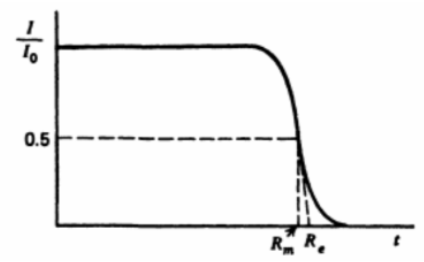
\includegraphics{alphaRadiation.png}
    \caption{
    אופיין איכותי של התנהגות עוצמת קרינת 
    $\alpha$
    במעבר בחומר ביחס למרחק.
    %TODO: explain R_m and R_e
    }
    \label{fig:alphaDecay}
\end{figure}

בנוסף
מדדנו את את הקשר בין עוצמת הקרינה למרחק מהגלאי.
כאשר הקשר התאורטי ניתן בנוסחא 
\ref{equ:distanceIntensity}.

\begin{equ}
$$I(r) = \frac{I_0}{r^2}$$
\caption{
היחס בין עוצמת הקרינה למרחק מן הגלאי עבור 
$I_0$ 
העוצמה המקסימלית.
}
\label{equ:distanceIntensity}
\end{equ}

חלקיקי ה
$\beta$
הם אלקטרונים שנפלטים מהאטום כאשר ניוטרון דועך והופך לניטרון אלקטרון וניוטרנו.
גם עבור חלקיק ה
$\beta$
נרצה למדוד את הדעיכה בעת מעבר דרך חומר.
בעזרת חוק
\textenglish{Beer-Lambert}
נוכל לקבל את היחס בין העוצמה לעובי החומר .

\begin{equ}
$$I = I_0 e^{-\mu t}$$
\caption{עוצמת הקרינה כתלות בעובי החומר בה היא עוברת כאשר
$\mu$
מקדם הדעיכה}
\end{equ}
\clearpage
\section{
מערכת הניסוי
}
מערכת הניסוי מוצגת באיור 
\ref{fig:systemSetupNuclear}.
המערכת מורכבת ממונה גייגר, אפליקציה שבעזרתה ניתן למדוד את מספר הקריאות שהמונה קיבל בזמן נתון,
וחוסמי קרינה מסוגים ועוביים שונים.

% TODO: add ref to the guide
\begin{figure}[ht!]
    \centering
    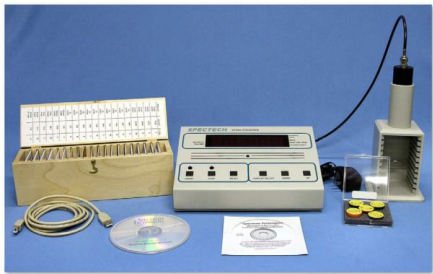
\includegraphics{systemSetup.png}
    \caption{
    מערכת הניסוי.
    \cite{Manual}
    }
    \label{fig:systemSetupNuclear}
\end{figure}

מונה גייגר בנוי משפופרת גלילית מוליכה בעלת חלון כניסה דק. השפופרת משמשת כקתודה ומכילה בתוכה אנודה העשויה מחוט מוליך הנמצא במתח גבוה ומבודד מהדפנות.
בתוך השפורפרת מצוי גז אציל, כך בעת כניסת קרינה לתא היא מיננת את הגז.
המטען נאסף בתיל החיובי, וכאשר הוא זורם חזרה לדפנות, נרשמת במערכת פעימה שמעידה על אירוע. המכשיר מגביר את האות ומציג אותו למשתמש.

לאחר היינון חלה רגיעה,
האלקטרונים והאטומים מתלכדים מחדש בזמן המכונה זמן ההתלכדות. בטווח זמנים זה המכשיר אינו מסוגל להוציא אותות נוספים.

כיוצא מן הכתוב, כמות הפעימות תלויה במתח המסופק. בגרף
\ref{fig:plateau}
מוצג יחס זה.

\begin{figure}[ht!]
    \centering
    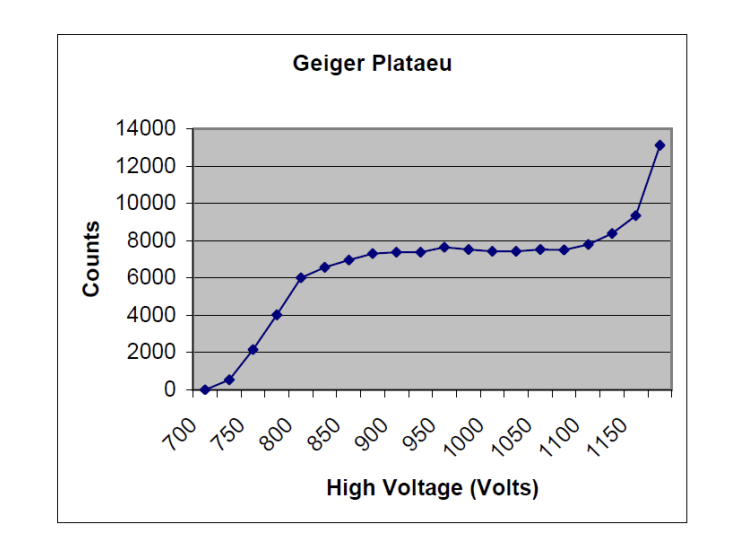
\includegraphics{plateau.png}
    \caption{כמות הפעימות כתלות במתח במונה גייגר, לקוח מהתדריך}
    \label{fig:plateau}
\end{figure}

מתח העבודה הרצוי יהיה בתחום ה
\textenglish{"plateau"},
בו כמות הפעימות בקירוב איננה משתנה כתלות במתח.

\section{
תוצאות
}

\subsection{
מדידת דעיכת בטא
}

% TODO: Explain this

\begin{graph}[ht!]
    \centering
    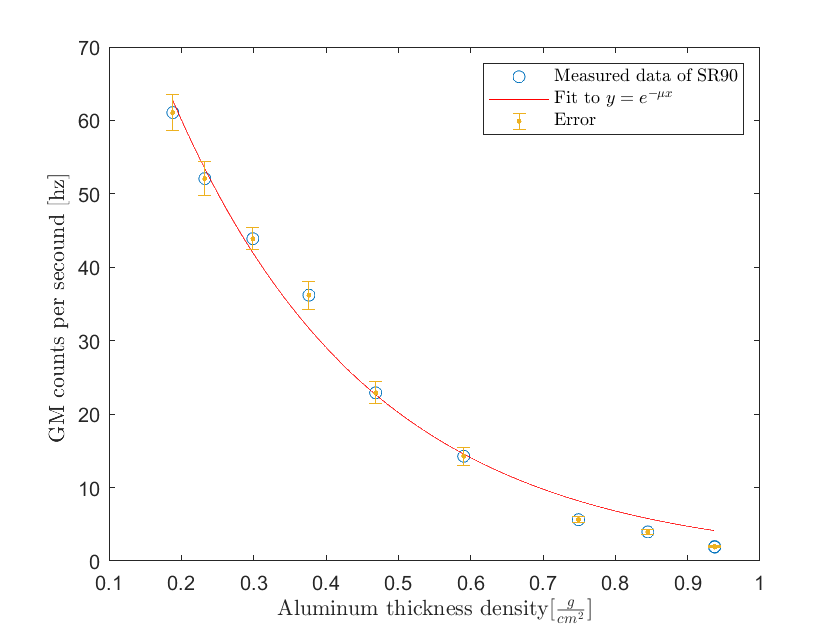
\includegraphics[width=0.79\textwidth]{SR90.png}
    \caption{
    % TODO
    }
    \label{graph:decay_SR90}
\end{graph}

\begin{graph}[ht!]
    \centering
    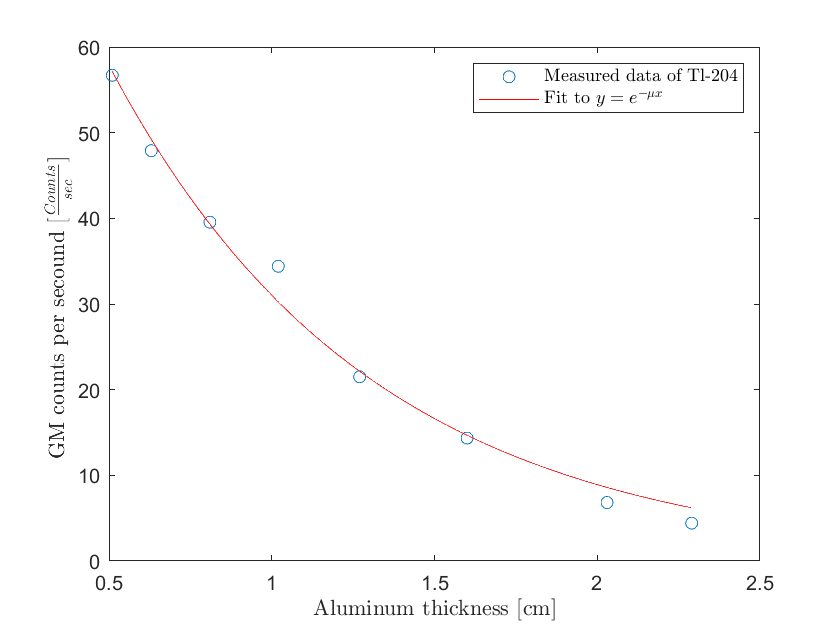
\includegraphics[width=0.79\textwidth]{Tl-204.png}
    \caption{
    % TODO
    }
    \label{graph:decay_Tl-204}
\end{graph}

\subsection{
מדידת דעיכת עוצמת קרינה כתלות במרחק
}

עבור
\textenglish{Thalium-204}
ועבור
\textenglish{Strontium-90}
מדדנו את הקשר בין עוצמת הקרינה הרדיואקטיבית למרחק של המקור הרדיואקטיבי מהגלאי. ביצענו התאמה לביטוי דומה לביטוי במשוואה
\ref{equ:distanceIntensity}:

\begin{equ}
$$ I(r) \sim \frac{1}{(r+a)^2}$$
\label{equ:distanceIntensity_fit}
\end{equ}

ביצענו התאמה לפונקציה זו כי לא הייתה באפשרותינו למדוד את המרחק בין המקור לגלאי באופן אבסולוטי, אלא רק באופן יחסי. התוצאות מוצגות בגרפים

\begin{graph}[H]
	\begin{center}
	\resizebox{\textwidth}{!}{%% Creator: Matplotlib, PGF backend
%%
%% To include the figure in your LaTeX document, write
%%   \input{<filename>.pgf}
%%
%% Make sure the required packages are loaded in your preamble
%%   \usepackage{pgf}
%%
%% Also ensure that all the required font packages are loaded; for instance,
%% the lmodern package is sometimes necessary when using math font.
%%   \usepackage{lmodern}
%%
%% Figures using additional raster images can only be included by \input if
%% they are in the same directory as the main LaTeX file. For loading figures
%% from other directories you can use the `import` package
%%   \usepackage{import}
%%
%% and then include the figures with
%%   \import{<path to file>}{<filename>.pgf}
%%
%% Matplotlib used the following preamble
%%   \usepackage{fontspec}
%%   \setmainfont{DejaVuSerif.ttf}[Path=\detokenize{/nix/store/y1lz1xbv947zrmpgy95md6sq0ryp2rsg-python3.9-matplotlib-3.5.1/lib/python3.9/site-packages/matplotlib/mpl-data/fonts/ttf/}]
%%   \setsansfont{DejaVuSans.ttf}[Path=\detokenize{/nix/store/y1lz1xbv947zrmpgy95md6sq0ryp2rsg-python3.9-matplotlib-3.5.1/lib/python3.9/site-packages/matplotlib/mpl-data/fonts/ttf/}]
%%   \setmonofont{DejaVuSansMono.ttf}[Path=\detokenize{/nix/store/y1lz1xbv947zrmpgy95md6sq0ryp2rsg-python3.9-matplotlib-3.5.1/lib/python3.9/site-packages/matplotlib/mpl-data/fonts/ttf/}]
%%
\begingroup%
\makeatletter%
\begin{pgfpicture}%
\pgfpathrectangle{\pgfpointorigin}{\pgfqpoint{6.400000in}{4.800000in}}%
\pgfusepath{use as bounding box, clip}%
\begin{pgfscope}%
\pgfsetbuttcap%
\pgfsetmiterjoin%
\definecolor{currentfill}{rgb}{1.000000,1.000000,1.000000}%
\pgfsetfillcolor{currentfill}%
\pgfsetlinewidth{0.000000pt}%
\definecolor{currentstroke}{rgb}{1.000000,1.000000,1.000000}%
\pgfsetstrokecolor{currentstroke}%
\pgfsetdash{}{0pt}%
\pgfpathmoveto{\pgfqpoint{0.000000in}{0.000000in}}%
\pgfpathlineto{\pgfqpoint{6.400000in}{0.000000in}}%
\pgfpathlineto{\pgfqpoint{6.400000in}{4.800000in}}%
\pgfpathlineto{\pgfqpoint{0.000000in}{4.800000in}}%
\pgfpathlineto{\pgfqpoint{0.000000in}{0.000000in}}%
\pgfpathclose%
\pgfusepath{fill}%
\end{pgfscope}%
\begin{pgfscope}%
\pgfsetbuttcap%
\pgfsetmiterjoin%
\definecolor{currentfill}{rgb}{1.000000,1.000000,1.000000}%
\pgfsetfillcolor{currentfill}%
\pgfsetlinewidth{0.000000pt}%
\definecolor{currentstroke}{rgb}{0.000000,0.000000,0.000000}%
\pgfsetstrokecolor{currentstroke}%
\pgfsetstrokeopacity{0.000000}%
\pgfsetdash{}{0pt}%
\pgfpathmoveto{\pgfqpoint{0.800000in}{0.528000in}}%
\pgfpathlineto{\pgfqpoint{5.760000in}{0.528000in}}%
\pgfpathlineto{\pgfqpoint{5.760000in}{4.224000in}}%
\pgfpathlineto{\pgfqpoint{0.800000in}{4.224000in}}%
\pgfpathlineto{\pgfqpoint{0.800000in}{0.528000in}}%
\pgfpathclose%
\pgfusepath{fill}%
\end{pgfscope}%
\begin{pgfscope}%
\pgfsetbuttcap%
\pgfsetroundjoin%
\definecolor{currentfill}{rgb}{0.000000,0.000000,0.000000}%
\pgfsetfillcolor{currentfill}%
\pgfsetlinewidth{0.803000pt}%
\definecolor{currentstroke}{rgb}{0.000000,0.000000,0.000000}%
\pgfsetstrokecolor{currentstroke}%
\pgfsetdash{}{0pt}%
\pgfsys@defobject{currentmarker}{\pgfqpoint{0.000000in}{-0.048611in}}{\pgfqpoint{0.000000in}{0.000000in}}{%
\pgfpathmoveto{\pgfqpoint{0.000000in}{0.000000in}}%
\pgfpathlineto{\pgfqpoint{0.000000in}{-0.048611in}}%
\pgfusepath{stroke,fill}%
}%
\begin{pgfscope}%
\pgfsys@transformshift{1.564585in}{0.528000in}%
\pgfsys@useobject{currentmarker}{}%
\end{pgfscope}%
\end{pgfscope}%
\begin{pgfscope}%
\definecolor{textcolor}{rgb}{0.000000,0.000000,0.000000}%
\pgfsetstrokecolor{textcolor}%
\pgfsetfillcolor{textcolor}%
\pgftext[x=1.564585in,y=0.430778in,,top]{\color{textcolor}\sffamily\fontsize{10.000000}{12.000000}\selectfont \(\displaystyle {2}\)}%
\end{pgfscope}%
\begin{pgfscope}%
\pgfsetbuttcap%
\pgfsetroundjoin%
\definecolor{currentfill}{rgb}{0.000000,0.000000,0.000000}%
\pgfsetfillcolor{currentfill}%
\pgfsetlinewidth{0.803000pt}%
\definecolor{currentstroke}{rgb}{0.000000,0.000000,0.000000}%
\pgfsetstrokecolor{currentstroke}%
\pgfsetdash{}{0pt}%
\pgfsys@defobject{currentmarker}{\pgfqpoint{0.000000in}{-0.048611in}}{\pgfqpoint{0.000000in}{0.000000in}}{%
\pgfpathmoveto{\pgfqpoint{0.000000in}{0.000000in}}%
\pgfpathlineto{\pgfqpoint{0.000000in}{-0.048611in}}%
\pgfusepath{stroke,fill}%
}%
\begin{pgfscope}%
\pgfsys@transformshift{2.544822in}{0.528000in}%
\pgfsys@useobject{currentmarker}{}%
\end{pgfscope}%
\end{pgfscope}%
\begin{pgfscope}%
\definecolor{textcolor}{rgb}{0.000000,0.000000,0.000000}%
\pgfsetstrokecolor{textcolor}%
\pgfsetfillcolor{textcolor}%
\pgftext[x=2.544822in,y=0.430778in,,top]{\color{textcolor}\sffamily\fontsize{10.000000}{12.000000}\selectfont \(\displaystyle {4}\)}%
\end{pgfscope}%
\begin{pgfscope}%
\pgfsetbuttcap%
\pgfsetroundjoin%
\definecolor{currentfill}{rgb}{0.000000,0.000000,0.000000}%
\pgfsetfillcolor{currentfill}%
\pgfsetlinewidth{0.803000pt}%
\definecolor{currentstroke}{rgb}{0.000000,0.000000,0.000000}%
\pgfsetstrokecolor{currentstroke}%
\pgfsetdash{}{0pt}%
\pgfsys@defobject{currentmarker}{\pgfqpoint{0.000000in}{-0.048611in}}{\pgfqpoint{0.000000in}{0.000000in}}{%
\pgfpathmoveto{\pgfqpoint{0.000000in}{0.000000in}}%
\pgfpathlineto{\pgfqpoint{0.000000in}{-0.048611in}}%
\pgfusepath{stroke,fill}%
}%
\begin{pgfscope}%
\pgfsys@transformshift{3.525059in}{0.528000in}%
\pgfsys@useobject{currentmarker}{}%
\end{pgfscope}%
\end{pgfscope}%
\begin{pgfscope}%
\definecolor{textcolor}{rgb}{0.000000,0.000000,0.000000}%
\pgfsetstrokecolor{textcolor}%
\pgfsetfillcolor{textcolor}%
\pgftext[x=3.525059in,y=0.430778in,,top]{\color{textcolor}\sffamily\fontsize{10.000000}{12.000000}\selectfont \(\displaystyle {6}\)}%
\end{pgfscope}%
\begin{pgfscope}%
\pgfsetbuttcap%
\pgfsetroundjoin%
\definecolor{currentfill}{rgb}{0.000000,0.000000,0.000000}%
\pgfsetfillcolor{currentfill}%
\pgfsetlinewidth{0.803000pt}%
\definecolor{currentstroke}{rgb}{0.000000,0.000000,0.000000}%
\pgfsetstrokecolor{currentstroke}%
\pgfsetdash{}{0pt}%
\pgfsys@defobject{currentmarker}{\pgfqpoint{0.000000in}{-0.048611in}}{\pgfqpoint{0.000000in}{0.000000in}}{%
\pgfpathmoveto{\pgfqpoint{0.000000in}{0.000000in}}%
\pgfpathlineto{\pgfqpoint{0.000000in}{-0.048611in}}%
\pgfusepath{stroke,fill}%
}%
\begin{pgfscope}%
\pgfsys@transformshift{4.505296in}{0.528000in}%
\pgfsys@useobject{currentmarker}{}%
\end{pgfscope}%
\end{pgfscope}%
\begin{pgfscope}%
\definecolor{textcolor}{rgb}{0.000000,0.000000,0.000000}%
\pgfsetstrokecolor{textcolor}%
\pgfsetfillcolor{textcolor}%
\pgftext[x=4.505296in,y=0.430778in,,top]{\color{textcolor}\sffamily\fontsize{10.000000}{12.000000}\selectfont \(\displaystyle {8}\)}%
\end{pgfscope}%
\begin{pgfscope}%
\pgfsetbuttcap%
\pgfsetroundjoin%
\definecolor{currentfill}{rgb}{0.000000,0.000000,0.000000}%
\pgfsetfillcolor{currentfill}%
\pgfsetlinewidth{0.803000pt}%
\definecolor{currentstroke}{rgb}{0.000000,0.000000,0.000000}%
\pgfsetstrokecolor{currentstroke}%
\pgfsetdash{}{0pt}%
\pgfsys@defobject{currentmarker}{\pgfqpoint{0.000000in}{-0.048611in}}{\pgfqpoint{0.000000in}{0.000000in}}{%
\pgfpathmoveto{\pgfqpoint{0.000000in}{0.000000in}}%
\pgfpathlineto{\pgfqpoint{0.000000in}{-0.048611in}}%
\pgfusepath{stroke,fill}%
}%
\begin{pgfscope}%
\pgfsys@transformshift{5.485534in}{0.528000in}%
\pgfsys@useobject{currentmarker}{}%
\end{pgfscope}%
\end{pgfscope}%
\begin{pgfscope}%
\definecolor{textcolor}{rgb}{0.000000,0.000000,0.000000}%
\pgfsetstrokecolor{textcolor}%
\pgfsetfillcolor{textcolor}%
\pgftext[x=5.485534in,y=0.430778in,,top]{\color{textcolor}\sffamily\fontsize{10.000000}{12.000000}\selectfont \(\displaystyle {10}\)}%
\end{pgfscope}%
\begin{pgfscope}%
\definecolor{textcolor}{rgb}{0.000000,0.000000,0.000000}%
\pgfsetstrokecolor{textcolor}%
\pgfsetfillcolor{textcolor}%
\pgftext[x=3.280000in,y=0.240809in,,top]{\color{textcolor}\sffamily\fontsize{10.000000}{12.000000}\selectfont Relative Distance [cm]}%
\end{pgfscope}%
\begin{pgfscope}%
\pgfsetbuttcap%
\pgfsetroundjoin%
\definecolor{currentfill}{rgb}{0.000000,0.000000,0.000000}%
\pgfsetfillcolor{currentfill}%
\pgfsetlinewidth{0.803000pt}%
\definecolor{currentstroke}{rgb}{0.000000,0.000000,0.000000}%
\pgfsetstrokecolor{currentstroke}%
\pgfsetdash{}{0pt}%
\pgfsys@defobject{currentmarker}{\pgfqpoint{-0.048611in}{0.000000in}}{\pgfqpoint{-0.000000in}{0.000000in}}{%
\pgfpathmoveto{\pgfqpoint{-0.000000in}{0.000000in}}%
\pgfpathlineto{\pgfqpoint{-0.048611in}{0.000000in}}%
\pgfusepath{stroke,fill}%
}%
\begin{pgfscope}%
\pgfsys@transformshift{0.800000in}{1.016984in}%
\pgfsys@useobject{currentmarker}{}%
\end{pgfscope}%
\end{pgfscope}%
\begin{pgfscope}%
\definecolor{textcolor}{rgb}{0.000000,0.000000,0.000000}%
\pgfsetstrokecolor{textcolor}%
\pgfsetfillcolor{textcolor}%
\pgftext[x=0.563888in, y=0.964222in, left, base]{\color{textcolor}\sffamily\fontsize{10.000000}{12.000000}\selectfont \(\displaystyle {50}\)}%
\end{pgfscope}%
\begin{pgfscope}%
\pgfsetbuttcap%
\pgfsetroundjoin%
\definecolor{currentfill}{rgb}{0.000000,0.000000,0.000000}%
\pgfsetfillcolor{currentfill}%
\pgfsetlinewidth{0.803000pt}%
\definecolor{currentstroke}{rgb}{0.000000,0.000000,0.000000}%
\pgfsetstrokecolor{currentstroke}%
\pgfsetdash{}{0pt}%
\pgfsys@defobject{currentmarker}{\pgfqpoint{-0.048611in}{0.000000in}}{\pgfqpoint{-0.000000in}{0.000000in}}{%
\pgfpathmoveto{\pgfqpoint{-0.000000in}{0.000000in}}%
\pgfpathlineto{\pgfqpoint{-0.048611in}{0.000000in}}%
\pgfusepath{stroke,fill}%
}%
\begin{pgfscope}%
\pgfsys@transformshift{0.800000in}{1.509726in}%
\pgfsys@useobject{currentmarker}{}%
\end{pgfscope}%
\end{pgfscope}%
\begin{pgfscope}%
\definecolor{textcolor}{rgb}{0.000000,0.000000,0.000000}%
\pgfsetstrokecolor{textcolor}%
\pgfsetfillcolor{textcolor}%
\pgftext[x=0.494444in, y=1.456964in, left, base]{\color{textcolor}\sffamily\fontsize{10.000000}{12.000000}\selectfont \(\displaystyle {100}\)}%
\end{pgfscope}%
\begin{pgfscope}%
\pgfsetbuttcap%
\pgfsetroundjoin%
\definecolor{currentfill}{rgb}{0.000000,0.000000,0.000000}%
\pgfsetfillcolor{currentfill}%
\pgfsetlinewidth{0.803000pt}%
\definecolor{currentstroke}{rgb}{0.000000,0.000000,0.000000}%
\pgfsetstrokecolor{currentstroke}%
\pgfsetdash{}{0pt}%
\pgfsys@defobject{currentmarker}{\pgfqpoint{-0.048611in}{0.000000in}}{\pgfqpoint{-0.000000in}{0.000000in}}{%
\pgfpathmoveto{\pgfqpoint{-0.000000in}{0.000000in}}%
\pgfpathlineto{\pgfqpoint{-0.048611in}{0.000000in}}%
\pgfusepath{stroke,fill}%
}%
\begin{pgfscope}%
\pgfsys@transformshift{0.800000in}{2.002468in}%
\pgfsys@useobject{currentmarker}{}%
\end{pgfscope}%
\end{pgfscope}%
\begin{pgfscope}%
\definecolor{textcolor}{rgb}{0.000000,0.000000,0.000000}%
\pgfsetstrokecolor{textcolor}%
\pgfsetfillcolor{textcolor}%
\pgftext[x=0.494444in, y=1.949707in, left, base]{\color{textcolor}\sffamily\fontsize{10.000000}{12.000000}\selectfont \(\displaystyle {150}\)}%
\end{pgfscope}%
\begin{pgfscope}%
\pgfsetbuttcap%
\pgfsetroundjoin%
\definecolor{currentfill}{rgb}{0.000000,0.000000,0.000000}%
\pgfsetfillcolor{currentfill}%
\pgfsetlinewidth{0.803000pt}%
\definecolor{currentstroke}{rgb}{0.000000,0.000000,0.000000}%
\pgfsetstrokecolor{currentstroke}%
\pgfsetdash{}{0pt}%
\pgfsys@defobject{currentmarker}{\pgfqpoint{-0.048611in}{0.000000in}}{\pgfqpoint{-0.000000in}{0.000000in}}{%
\pgfpathmoveto{\pgfqpoint{-0.000000in}{0.000000in}}%
\pgfpathlineto{\pgfqpoint{-0.048611in}{0.000000in}}%
\pgfusepath{stroke,fill}%
}%
\begin{pgfscope}%
\pgfsys@transformshift{0.800000in}{2.495211in}%
\pgfsys@useobject{currentmarker}{}%
\end{pgfscope}%
\end{pgfscope}%
\begin{pgfscope}%
\definecolor{textcolor}{rgb}{0.000000,0.000000,0.000000}%
\pgfsetstrokecolor{textcolor}%
\pgfsetfillcolor{textcolor}%
\pgftext[x=0.494444in, y=2.442449in, left, base]{\color{textcolor}\sffamily\fontsize{10.000000}{12.000000}\selectfont \(\displaystyle {200}\)}%
\end{pgfscope}%
\begin{pgfscope}%
\pgfsetbuttcap%
\pgfsetroundjoin%
\definecolor{currentfill}{rgb}{0.000000,0.000000,0.000000}%
\pgfsetfillcolor{currentfill}%
\pgfsetlinewidth{0.803000pt}%
\definecolor{currentstroke}{rgb}{0.000000,0.000000,0.000000}%
\pgfsetstrokecolor{currentstroke}%
\pgfsetdash{}{0pt}%
\pgfsys@defobject{currentmarker}{\pgfqpoint{-0.048611in}{0.000000in}}{\pgfqpoint{-0.000000in}{0.000000in}}{%
\pgfpathmoveto{\pgfqpoint{-0.000000in}{0.000000in}}%
\pgfpathlineto{\pgfqpoint{-0.048611in}{0.000000in}}%
\pgfusepath{stroke,fill}%
}%
\begin{pgfscope}%
\pgfsys@transformshift{0.800000in}{2.987953in}%
\pgfsys@useobject{currentmarker}{}%
\end{pgfscope}%
\end{pgfscope}%
\begin{pgfscope}%
\definecolor{textcolor}{rgb}{0.000000,0.000000,0.000000}%
\pgfsetstrokecolor{textcolor}%
\pgfsetfillcolor{textcolor}%
\pgftext[x=0.494444in, y=2.935192in, left, base]{\color{textcolor}\sffamily\fontsize{10.000000}{12.000000}\selectfont \(\displaystyle {250}\)}%
\end{pgfscope}%
\begin{pgfscope}%
\pgfsetbuttcap%
\pgfsetroundjoin%
\definecolor{currentfill}{rgb}{0.000000,0.000000,0.000000}%
\pgfsetfillcolor{currentfill}%
\pgfsetlinewidth{0.803000pt}%
\definecolor{currentstroke}{rgb}{0.000000,0.000000,0.000000}%
\pgfsetstrokecolor{currentstroke}%
\pgfsetdash{}{0pt}%
\pgfsys@defobject{currentmarker}{\pgfqpoint{-0.048611in}{0.000000in}}{\pgfqpoint{-0.000000in}{0.000000in}}{%
\pgfpathmoveto{\pgfqpoint{-0.000000in}{0.000000in}}%
\pgfpathlineto{\pgfqpoint{-0.048611in}{0.000000in}}%
\pgfusepath{stroke,fill}%
}%
\begin{pgfscope}%
\pgfsys@transformshift{0.800000in}{3.480696in}%
\pgfsys@useobject{currentmarker}{}%
\end{pgfscope}%
\end{pgfscope}%
\begin{pgfscope}%
\definecolor{textcolor}{rgb}{0.000000,0.000000,0.000000}%
\pgfsetstrokecolor{textcolor}%
\pgfsetfillcolor{textcolor}%
\pgftext[x=0.494444in, y=3.427934in, left, base]{\color{textcolor}\sffamily\fontsize{10.000000}{12.000000}\selectfont \(\displaystyle {300}\)}%
\end{pgfscope}%
\begin{pgfscope}%
\pgfsetbuttcap%
\pgfsetroundjoin%
\definecolor{currentfill}{rgb}{0.000000,0.000000,0.000000}%
\pgfsetfillcolor{currentfill}%
\pgfsetlinewidth{0.803000pt}%
\definecolor{currentstroke}{rgb}{0.000000,0.000000,0.000000}%
\pgfsetstrokecolor{currentstroke}%
\pgfsetdash{}{0pt}%
\pgfsys@defobject{currentmarker}{\pgfqpoint{-0.048611in}{0.000000in}}{\pgfqpoint{-0.000000in}{0.000000in}}{%
\pgfpathmoveto{\pgfqpoint{-0.000000in}{0.000000in}}%
\pgfpathlineto{\pgfqpoint{-0.048611in}{0.000000in}}%
\pgfusepath{stroke,fill}%
}%
\begin{pgfscope}%
\pgfsys@transformshift{0.800000in}{3.973438in}%
\pgfsys@useobject{currentmarker}{}%
\end{pgfscope}%
\end{pgfscope}%
\begin{pgfscope}%
\definecolor{textcolor}{rgb}{0.000000,0.000000,0.000000}%
\pgfsetstrokecolor{textcolor}%
\pgfsetfillcolor{textcolor}%
\pgftext[x=0.494444in, y=3.920677in, left, base]{\color{textcolor}\sffamily\fontsize{10.000000}{12.000000}\selectfont \(\displaystyle {350}\)}%
\end{pgfscope}%
\begin{pgfscope}%
\definecolor{textcolor}{rgb}{0.000000,0.000000,0.000000}%
\pgfsetstrokecolor{textcolor}%
\pgfsetfillcolor{textcolor}%
\pgftext[x=0.438888in,y=2.376000in,,bottom,rotate=90.000000]{\color{textcolor}\sffamily\fontsize{10.000000}{12.000000}\selectfont Counts [Hz]}%
\end{pgfscope}%
\begin{pgfscope}%
\pgfpathrectangle{\pgfqpoint{0.800000in}{0.528000in}}{\pgfqpoint{4.960000in}{3.696000in}}%
\pgfusepath{clip}%
\pgfsetbuttcap%
\pgfsetroundjoin%
\pgfsetlinewidth{1.505625pt}%
\definecolor{currentstroke}{rgb}{0.121569,0.466667,0.705882}%
\pgfsetstrokecolor{currentstroke}%
\pgfsetdash{}{0pt}%
\pgfpathmoveto{\pgfqpoint{1.025455in}{3.909382in}}%
\pgfpathlineto{\pgfqpoint{1.123478in}{3.909382in}}%
\pgfusepath{stroke}%
\end{pgfscope}%
\begin{pgfscope}%
\pgfpathrectangle{\pgfqpoint{0.800000in}{0.528000in}}{\pgfqpoint{4.960000in}{3.696000in}}%
\pgfusepath{clip}%
\pgfsetbuttcap%
\pgfsetroundjoin%
\pgfsetlinewidth{1.505625pt}%
\definecolor{currentstroke}{rgb}{0.121569,0.466667,0.705882}%
\pgfsetstrokecolor{currentstroke}%
\pgfsetdash{}{0pt}%
\pgfpathmoveto{\pgfqpoint{1.515573in}{2.405532in}}%
\pgfpathlineto{\pgfqpoint{1.613597in}{2.405532in}}%
\pgfusepath{stroke}%
\end{pgfscope}%
\begin{pgfscope}%
\pgfpathrectangle{\pgfqpoint{0.800000in}{0.528000in}}{\pgfqpoint{4.960000in}{3.696000in}}%
\pgfusepath{clip}%
\pgfsetbuttcap%
\pgfsetroundjoin%
\pgfsetlinewidth{1.505625pt}%
\definecolor{currentstroke}{rgb}{0.121569,0.466667,0.705882}%
\pgfsetstrokecolor{currentstroke}%
\pgfsetdash{}{0pt}%
\pgfpathmoveto{\pgfqpoint{2.005692in}{1.684157in}}%
\pgfpathlineto{\pgfqpoint{2.103715in}{1.684157in}}%
\pgfusepath{stroke}%
\end{pgfscope}%
\begin{pgfscope}%
\pgfpathrectangle{\pgfqpoint{0.800000in}{0.528000in}}{\pgfqpoint{4.960000in}{3.696000in}}%
\pgfusepath{clip}%
\pgfsetbuttcap%
\pgfsetroundjoin%
\pgfsetlinewidth{1.505625pt}%
\definecolor{currentstroke}{rgb}{0.121569,0.466667,0.705882}%
\pgfsetstrokecolor{currentstroke}%
\pgfsetdash{}{0pt}%
\pgfpathmoveto{\pgfqpoint{2.495810in}{1.292919in}}%
\pgfpathlineto{\pgfqpoint{2.593834in}{1.292919in}}%
\pgfusepath{stroke}%
\end{pgfscope}%
\begin{pgfscope}%
\pgfpathrectangle{\pgfqpoint{0.800000in}{0.528000in}}{\pgfqpoint{4.960000in}{3.696000in}}%
\pgfusepath{clip}%
\pgfsetbuttcap%
\pgfsetroundjoin%
\pgfsetlinewidth{1.505625pt}%
\definecolor{currentstroke}{rgb}{0.121569,0.466667,0.705882}%
\pgfsetstrokecolor{currentstroke}%
\pgfsetdash{}{0pt}%
\pgfpathmoveto{\pgfqpoint{2.985929in}{1.086953in}}%
\pgfpathlineto{\pgfqpoint{3.083953in}{1.086953in}}%
\pgfusepath{stroke}%
\end{pgfscope}%
\begin{pgfscope}%
\pgfpathrectangle{\pgfqpoint{0.800000in}{0.528000in}}{\pgfqpoint{4.960000in}{3.696000in}}%
\pgfusepath{clip}%
\pgfsetbuttcap%
\pgfsetroundjoin%
\pgfsetlinewidth{1.505625pt}%
\definecolor{currentstroke}{rgb}{0.121569,0.466667,0.705882}%
\pgfsetstrokecolor{currentstroke}%
\pgfsetdash{}{0pt}%
\pgfpathmoveto{\pgfqpoint{3.476047in}{0.927304in}}%
\pgfpathlineto{\pgfqpoint{3.574071in}{0.927304in}}%
\pgfusepath{stroke}%
\end{pgfscope}%
\begin{pgfscope}%
\pgfpathrectangle{\pgfqpoint{0.800000in}{0.528000in}}{\pgfqpoint{4.960000in}{3.696000in}}%
\pgfusepath{clip}%
\pgfsetbuttcap%
\pgfsetroundjoin%
\pgfsetlinewidth{1.505625pt}%
\definecolor{currentstroke}{rgb}{0.121569,0.466667,0.705882}%
\pgfsetstrokecolor{currentstroke}%
\pgfsetdash{}{0pt}%
\pgfpathmoveto{\pgfqpoint{3.966166in}{0.882958in}}%
\pgfpathlineto{\pgfqpoint{4.064190in}{0.882958in}}%
\pgfusepath{stroke}%
\end{pgfscope}%
\begin{pgfscope}%
\pgfpathrectangle{\pgfqpoint{0.800000in}{0.528000in}}{\pgfqpoint{4.960000in}{3.696000in}}%
\pgfusepath{clip}%
\pgfsetbuttcap%
\pgfsetroundjoin%
\pgfsetlinewidth{1.505625pt}%
\definecolor{currentstroke}{rgb}{0.121569,0.466667,0.705882}%
\pgfsetstrokecolor{currentstroke}%
\pgfsetdash{}{0pt}%
\pgfpathmoveto{\pgfqpoint{4.456285in}{0.778496in}}%
\pgfpathlineto{\pgfqpoint{4.554308in}{0.778496in}}%
\pgfusepath{stroke}%
\end{pgfscope}%
\begin{pgfscope}%
\pgfpathrectangle{\pgfqpoint{0.800000in}{0.528000in}}{\pgfqpoint{4.960000in}{3.696000in}}%
\pgfusepath{clip}%
\pgfsetbuttcap%
\pgfsetroundjoin%
\pgfsetlinewidth{1.505625pt}%
\definecolor{currentstroke}{rgb}{0.121569,0.466667,0.705882}%
\pgfsetstrokecolor{currentstroke}%
\pgfsetdash{}{0pt}%
\pgfpathmoveto{\pgfqpoint{4.946403in}{0.757801in}}%
\pgfpathlineto{\pgfqpoint{5.044427in}{0.757801in}}%
\pgfusepath{stroke}%
\end{pgfscope}%
\begin{pgfscope}%
\pgfpathrectangle{\pgfqpoint{0.800000in}{0.528000in}}{\pgfqpoint{4.960000in}{3.696000in}}%
\pgfusepath{clip}%
\pgfsetbuttcap%
\pgfsetroundjoin%
\pgfsetlinewidth{1.505625pt}%
\definecolor{currentstroke}{rgb}{0.121569,0.466667,0.705882}%
\pgfsetstrokecolor{currentstroke}%
\pgfsetdash{}{0pt}%
\pgfpathmoveto{\pgfqpoint{5.436522in}{0.709512in}}%
\pgfpathlineto{\pgfqpoint{5.534545in}{0.709512in}}%
\pgfusepath{stroke}%
\end{pgfscope}%
\begin{pgfscope}%
\pgfpathrectangle{\pgfqpoint{0.800000in}{0.528000in}}{\pgfqpoint{4.960000in}{3.696000in}}%
\pgfusepath{clip}%
\pgfsetbuttcap%
\pgfsetroundjoin%
\pgfsetlinewidth{1.505625pt}%
\definecolor{currentstroke}{rgb}{0.121569,0.466667,0.705882}%
\pgfsetstrokecolor{currentstroke}%
\pgfsetdash{}{0pt}%
\pgfpathmoveto{\pgfqpoint{1.074466in}{3.851624in}}%
\pgfpathlineto{\pgfqpoint{1.074466in}{3.967140in}}%
\pgfusepath{stroke}%
\end{pgfscope}%
\begin{pgfscope}%
\pgfpathrectangle{\pgfqpoint{0.800000in}{0.528000in}}{\pgfqpoint{4.960000in}{3.696000in}}%
\pgfusepath{clip}%
\pgfsetbuttcap%
\pgfsetroundjoin%
\pgfsetlinewidth{1.505625pt}%
\definecolor{currentstroke}{rgb}{0.121569,0.466667,0.705882}%
\pgfsetstrokecolor{currentstroke}%
\pgfsetdash{}{0pt}%
\pgfpathmoveto{\pgfqpoint{1.564585in}{2.362474in}}%
\pgfpathlineto{\pgfqpoint{1.564585in}{2.448590in}}%
\pgfusepath{stroke}%
\end{pgfscope}%
\begin{pgfscope}%
\pgfpathrectangle{\pgfqpoint{0.800000in}{0.528000in}}{\pgfqpoint{4.960000in}{3.696000in}}%
\pgfusepath{clip}%
\pgfsetbuttcap%
\pgfsetroundjoin%
\pgfsetlinewidth{1.505625pt}%
\definecolor{currentstroke}{rgb}{0.121569,0.466667,0.705882}%
\pgfsetstrokecolor{currentstroke}%
\pgfsetdash{}{0pt}%
\pgfpathmoveto{\pgfqpoint{2.054704in}{1.650347in}}%
\pgfpathlineto{\pgfqpoint{2.054704in}{1.717966in}}%
\pgfusepath{stroke}%
\end{pgfscope}%
\begin{pgfscope}%
\pgfpathrectangle{\pgfqpoint{0.800000in}{0.528000in}}{\pgfqpoint{4.960000in}{3.696000in}}%
\pgfusepath{clip}%
\pgfsetbuttcap%
\pgfsetroundjoin%
\pgfsetlinewidth{1.505625pt}%
\definecolor{currentstroke}{rgb}{0.121569,0.466667,0.705882}%
\pgfsetstrokecolor{currentstroke}%
\pgfsetdash{}{0pt}%
\pgfpathmoveto{\pgfqpoint{2.544822in}{1.265396in}}%
\pgfpathlineto{\pgfqpoint{2.544822in}{1.320442in}}%
\pgfusepath{stroke}%
\end{pgfscope}%
\begin{pgfscope}%
\pgfpathrectangle{\pgfqpoint{0.800000in}{0.528000in}}{\pgfqpoint{4.960000in}{3.696000in}}%
\pgfusepath{clip}%
\pgfsetbuttcap%
\pgfsetroundjoin%
\pgfsetlinewidth{1.505625pt}%
\definecolor{currentstroke}{rgb}{0.121569,0.466667,0.705882}%
\pgfsetstrokecolor{currentstroke}%
\pgfsetdash{}{0pt}%
\pgfpathmoveto{\pgfqpoint{3.034941in}{1.063404in}}%
\pgfpathlineto{\pgfqpoint{3.034941in}{1.110502in}}%
\pgfusepath{stroke}%
\end{pgfscope}%
\begin{pgfscope}%
\pgfpathrectangle{\pgfqpoint{0.800000in}{0.528000in}}{\pgfqpoint{4.960000in}{3.696000in}}%
\pgfusepath{clip}%
\pgfsetbuttcap%
\pgfsetroundjoin%
\pgfsetlinewidth{1.505625pt}%
\definecolor{currentstroke}{rgb}{0.121569,0.466667,0.705882}%
\pgfsetstrokecolor{currentstroke}%
\pgfsetdash{}{0pt}%
\pgfpathmoveto{\pgfqpoint{3.525059in}{0.907374in}}%
\pgfpathlineto{\pgfqpoint{3.525059in}{0.947235in}}%
\pgfusepath{stroke}%
\end{pgfscope}%
\begin{pgfscope}%
\pgfpathrectangle{\pgfqpoint{0.800000in}{0.528000in}}{\pgfqpoint{4.960000in}{3.696000in}}%
\pgfusepath{clip}%
\pgfsetbuttcap%
\pgfsetroundjoin%
\pgfsetlinewidth{1.505625pt}%
\definecolor{currentstroke}{rgb}{0.121569,0.466667,0.705882}%
\pgfsetstrokecolor{currentstroke}%
\pgfsetdash{}{0pt}%
\pgfpathmoveto{\pgfqpoint{4.015178in}{0.864156in}}%
\pgfpathlineto{\pgfqpoint{4.015178in}{0.901759in}}%
\pgfusepath{stroke}%
\end{pgfscope}%
\begin{pgfscope}%
\pgfpathrectangle{\pgfqpoint{0.800000in}{0.528000in}}{\pgfqpoint{4.960000in}{3.696000in}}%
\pgfusepath{clip}%
\pgfsetbuttcap%
\pgfsetroundjoin%
\pgfsetlinewidth{1.505625pt}%
\definecolor{currentstroke}{rgb}{0.121569,0.466667,0.705882}%
\pgfsetstrokecolor{currentstroke}%
\pgfsetdash{}{0pt}%
\pgfpathmoveto{\pgfqpoint{4.505296in}{0.762667in}}%
\pgfpathlineto{\pgfqpoint{4.505296in}{0.794325in}}%
\pgfusepath{stroke}%
\end{pgfscope}%
\begin{pgfscope}%
\pgfpathrectangle{\pgfqpoint{0.800000in}{0.528000in}}{\pgfqpoint{4.960000in}{3.696000in}}%
\pgfusepath{clip}%
\pgfsetbuttcap%
\pgfsetroundjoin%
\pgfsetlinewidth{1.505625pt}%
\definecolor{currentstroke}{rgb}{0.121569,0.466667,0.705882}%
\pgfsetstrokecolor{currentstroke}%
\pgfsetdash{}{0pt}%
\pgfpathmoveto{\pgfqpoint{4.995415in}{0.742630in}}%
\pgfpathlineto{\pgfqpoint{4.995415in}{0.772972in}}%
\pgfusepath{stroke}%
\end{pgfscope}%
\begin{pgfscope}%
\pgfpathrectangle{\pgfqpoint{0.800000in}{0.528000in}}{\pgfqpoint{4.960000in}{3.696000in}}%
\pgfusepath{clip}%
\pgfsetbuttcap%
\pgfsetroundjoin%
\pgfsetlinewidth{1.505625pt}%
\definecolor{currentstroke}{rgb}{0.121569,0.466667,0.705882}%
\pgfsetstrokecolor{currentstroke}%
\pgfsetdash{}{0pt}%
\pgfpathmoveto{\pgfqpoint{5.485534in}{0.696000in}}%
\pgfpathlineto{\pgfqpoint{5.485534in}{0.723025in}}%
\pgfusepath{stroke}%
\end{pgfscope}%
\begin{pgfscope}%
\pgfpathrectangle{\pgfqpoint{0.800000in}{0.528000in}}{\pgfqpoint{4.960000in}{3.696000in}}%
\pgfusepath{clip}%
\pgfsetrectcap%
\pgfsetroundjoin%
\pgfsetlinewidth{1.505625pt}%
\definecolor{currentstroke}{rgb}{1.000000,0.498039,0.054902}%
\pgfsetstrokecolor{currentstroke}%
\pgfsetdash{}{0pt}%
\pgfpathmoveto{\pgfqpoint{1.074466in}{4.056000in}}%
\pgfpathlineto{\pgfqpoint{1.119023in}{3.667094in}}%
\pgfpathlineto{\pgfqpoint{1.163579in}{3.355396in}}%
\pgfpathlineto{\pgfqpoint{1.208135in}{3.099989in}}%
\pgfpathlineto{\pgfqpoint{1.252691in}{2.886888in}}%
\pgfpathlineto{\pgfqpoint{1.297248in}{2.706386in}}%
\pgfpathlineto{\pgfqpoint{1.341804in}{2.551533in}}%
\pgfpathlineto{\pgfqpoint{1.386360in}{2.417225in}}%
\pgfpathlineto{\pgfqpoint{1.430916in}{2.299628in}}%
\pgfpathlineto{\pgfqpoint{1.475473in}{2.195806in}}%
\pgfpathlineto{\pgfqpoint{1.520029in}{2.103473in}}%
\pgfpathlineto{\pgfqpoint{1.564585in}{2.020820in}}%
\pgfpathlineto{\pgfqpoint{1.609141in}{1.946402in}}%
\pgfpathlineto{\pgfqpoint{1.653697in}{1.879047in}}%
\pgfpathlineto{\pgfqpoint{1.698254in}{1.817794in}}%
\pgfpathlineto{\pgfqpoint{1.742810in}{1.761851in}}%
\pgfpathlineto{\pgfqpoint{1.787366in}{1.710555in}}%
\pgfpathlineto{\pgfqpoint{1.831922in}{1.663350in}}%
\pgfpathlineto{\pgfqpoint{1.876479in}{1.619767in}}%
\pgfpathlineto{\pgfqpoint{1.921035in}{1.579403in}}%
\pgfpathlineto{\pgfqpoint{1.965591in}{1.541914in}}%
\pgfpathlineto{\pgfqpoint{2.010147in}{1.507004in}}%
\pgfpathlineto{\pgfqpoint{2.054704in}{1.474416in}}%
\pgfpathlineto{\pgfqpoint{2.099260in}{1.443925in}}%
\pgfpathlineto{\pgfqpoint{2.143816in}{1.415335in}}%
\pgfpathlineto{\pgfqpoint{2.188372in}{1.388475in}}%
\pgfpathlineto{\pgfqpoint{2.232928in}{1.363191in}}%
\pgfpathlineto{\pgfqpoint{2.277485in}{1.339348in}}%
\pgfpathlineto{\pgfqpoint{2.322041in}{1.316828in}}%
\pgfpathlineto{\pgfqpoint{2.366597in}{1.295522in}}%
\pgfpathlineto{\pgfqpoint{2.411153in}{1.275335in}}%
\pgfpathlineto{\pgfqpoint{2.455710in}{1.256182in}}%
\pgfpathlineto{\pgfqpoint{2.500266in}{1.237985in}}%
\pgfpathlineto{\pgfqpoint{2.544822in}{1.220673in}}%
\pgfpathlineto{\pgfqpoint{2.589378in}{1.204185in}}%
\pgfpathlineto{\pgfqpoint{2.633935in}{1.188462in}}%
\pgfpathlineto{\pgfqpoint{2.678491in}{1.173453in}}%
\pgfpathlineto{\pgfqpoint{2.723047in}{1.159109in}}%
\pgfpathlineto{\pgfqpoint{2.767603in}{1.145388in}}%
\pgfpathlineto{\pgfqpoint{2.812160in}{1.132251in}}%
\pgfpathlineto{\pgfqpoint{2.856716in}{1.119659in}}%
\pgfpathlineto{\pgfqpoint{2.901272in}{1.107581in}}%
\pgfpathlineto{\pgfqpoint{2.945828in}{1.095986in}}%
\pgfpathlineto{\pgfqpoint{2.990384in}{1.084844in}}%
\pgfpathlineto{\pgfqpoint{3.034941in}{1.074130in}}%
\pgfpathlineto{\pgfqpoint{3.079497in}{1.063820in}}%
\pgfpathlineto{\pgfqpoint{3.124053in}{1.053891in}}%
\pgfpathlineto{\pgfqpoint{3.168609in}{1.044323in}}%
\pgfpathlineto{\pgfqpoint{3.213166in}{1.035096in}}%
\pgfpathlineto{\pgfqpoint{3.257722in}{1.026193in}}%
\pgfpathlineto{\pgfqpoint{3.302278in}{1.017596in}}%
\pgfpathlineto{\pgfqpoint{3.346834in}{1.009290in}}%
\pgfpathlineto{\pgfqpoint{3.391391in}{1.001261in}}%
\pgfpathlineto{\pgfqpoint{3.435947in}{0.993494in}}%
\pgfpathlineto{\pgfqpoint{3.480503in}{0.985978in}}%
\pgfpathlineto{\pgfqpoint{3.525059in}{0.978700in}}%
\pgfpathlineto{\pgfqpoint{3.569616in}{0.971650in}}%
\pgfpathlineto{\pgfqpoint{3.614172in}{0.964816in}}%
\pgfpathlineto{\pgfqpoint{3.658728in}{0.958189in}}%
\pgfpathlineto{\pgfqpoint{3.703284in}{0.951759in}}%
\pgfpathlineto{\pgfqpoint{3.747840in}{0.945519in}}%
\pgfpathlineto{\pgfqpoint{3.792397in}{0.939459in}}%
\pgfpathlineto{\pgfqpoint{3.836953in}{0.933572in}}%
\pgfpathlineto{\pgfqpoint{3.881509in}{0.927850in}}%
\pgfpathlineto{\pgfqpoint{3.926065in}{0.922288in}}%
\pgfpathlineto{\pgfqpoint{3.970622in}{0.916877in}}%
\pgfpathlineto{\pgfqpoint{4.015178in}{0.911613in}}%
\pgfpathlineto{\pgfqpoint{4.059734in}{0.906489in}}%
\pgfpathlineto{\pgfqpoint{4.104290in}{0.901500in}}%
\pgfpathlineto{\pgfqpoint{4.148847in}{0.896640in}}%
\pgfpathlineto{\pgfqpoint{4.193403in}{0.891905in}}%
\pgfpathlineto{\pgfqpoint{4.237959in}{0.887289in}}%
\pgfpathlineto{\pgfqpoint{4.282515in}{0.882789in}}%
\pgfpathlineto{\pgfqpoint{4.327072in}{0.878400in}}%
\pgfpathlineto{\pgfqpoint{4.371628in}{0.874117in}}%
\pgfpathlineto{\pgfqpoint{4.416184in}{0.869938in}}%
\pgfpathlineto{\pgfqpoint{4.460740in}{0.865858in}}%
\pgfpathlineto{\pgfqpoint{4.505296in}{0.861875in}}%
\pgfpathlineto{\pgfqpoint{4.549853in}{0.857983in}}%
\pgfpathlineto{\pgfqpoint{4.594409in}{0.854181in}}%
\pgfpathlineto{\pgfqpoint{4.638965in}{0.850466in}}%
\pgfpathlineto{\pgfqpoint{4.683521in}{0.846834in}}%
\pgfpathlineto{\pgfqpoint{4.728078in}{0.843282in}}%
\pgfpathlineto{\pgfqpoint{4.772634in}{0.839809in}}%
\pgfpathlineto{\pgfqpoint{4.817190in}{0.836411in}}%
\pgfpathlineto{\pgfqpoint{4.861746in}{0.833085in}}%
\pgfpathlineto{\pgfqpoint{4.906303in}{0.829831in}}%
\pgfpathlineto{\pgfqpoint{4.950859in}{0.826645in}}%
\pgfpathlineto{\pgfqpoint{4.995415in}{0.823526in}}%
\pgfpathlineto{\pgfqpoint{5.039971in}{0.820470in}}%
\pgfpathlineto{\pgfqpoint{5.084527in}{0.817477in}}%
\pgfpathlineto{\pgfqpoint{5.129084in}{0.814545in}}%
\pgfpathlineto{\pgfqpoint{5.173640in}{0.811671in}}%
\pgfpathlineto{\pgfqpoint{5.218196in}{0.808854in}}%
\pgfpathlineto{\pgfqpoint{5.262752in}{0.806092in}}%
\pgfpathlineto{\pgfqpoint{5.307309in}{0.803383in}}%
\pgfpathlineto{\pgfqpoint{5.351865in}{0.800727in}}%
\pgfpathlineto{\pgfqpoint{5.396421in}{0.798121in}}%
\pgfpathlineto{\pgfqpoint{5.440977in}{0.795565in}}%
\pgfpathlineto{\pgfqpoint{5.485534in}{0.793056in}}%
\pgfusepath{stroke}%
\end{pgfscope}%
\begin{pgfscope}%
\pgfpathrectangle{\pgfqpoint{0.800000in}{0.528000in}}{\pgfqpoint{4.960000in}{3.696000in}}%
\pgfusepath{clip}%
\pgfsetrectcap%
\pgfsetroundjoin%
\pgfsetlinewidth{1.505625pt}%
\definecolor{currentstroke}{rgb}{0.172549,0.627451,0.172549}%
\pgfsetstrokecolor{currentstroke}%
\pgfsetdash{}{0pt}%
\pgfpathmoveto{\pgfqpoint{1.074466in}{3.960031in}}%
\pgfpathlineto{\pgfqpoint{1.119023in}{3.647035in}}%
\pgfpathlineto{\pgfqpoint{1.163579in}{3.386343in}}%
\pgfpathlineto{\pgfqpoint{1.208135in}{3.165855in}}%
\pgfpathlineto{\pgfqpoint{1.252691in}{2.976936in}}%
\pgfpathlineto{\pgfqpoint{1.297248in}{2.813259in}}%
\pgfpathlineto{\pgfqpoint{1.341804in}{2.670082in}}%
\pgfpathlineto{\pgfqpoint{1.386360in}{2.543780in}}%
\pgfpathlineto{\pgfqpoint{1.430916in}{2.431537in}}%
\pgfpathlineto{\pgfqpoint{1.475473in}{2.331129in}}%
\pgfpathlineto{\pgfqpoint{1.520029in}{2.240777in}}%
\pgfpathlineto{\pgfqpoint{1.564585in}{2.159043in}}%
\pgfpathlineto{\pgfqpoint{1.609141in}{2.084749in}}%
\pgfpathlineto{\pgfqpoint{1.653697in}{2.016926in}}%
\pgfpathlineto{\pgfqpoint{1.698254in}{1.954761in}}%
\pgfpathlineto{\pgfqpoint{1.742810in}{1.897576in}}%
\pgfpathlineto{\pgfqpoint{1.787366in}{1.844795in}}%
\pgfpathlineto{\pgfqpoint{1.831922in}{1.795928in}}%
\pgfpathlineto{\pgfqpoint{1.876479in}{1.750556in}}%
\pgfpathlineto{\pgfqpoint{1.921035in}{1.708316in}}%
\pgfpathlineto{\pgfqpoint{1.965591in}{1.668896in}}%
\pgfpathlineto{\pgfqpoint{2.010147in}{1.632021in}}%
\pgfpathlineto{\pgfqpoint{2.054704in}{1.597453in}}%
\pgfpathlineto{\pgfqpoint{2.099260in}{1.564982in}}%
\pgfpathlineto{\pgfqpoint{2.143816in}{1.534423in}}%
\pgfpathlineto{\pgfqpoint{2.188372in}{1.505611in}}%
\pgfpathlineto{\pgfqpoint{2.232928in}{1.478402in}}%
\pgfpathlineto{\pgfqpoint{2.277485in}{1.452665in}}%
\pgfpathlineto{\pgfqpoint{2.322041in}{1.428283in}}%
\pgfpathlineto{\pgfqpoint{2.366597in}{1.405153in}}%
\pgfpathlineto{\pgfqpoint{2.411153in}{1.383180in}}%
\pgfpathlineto{\pgfqpoint{2.455710in}{1.362280in}}%
\pgfpathlineto{\pgfqpoint{2.500266in}{1.342376in}}%
\pgfpathlineto{\pgfqpoint{2.544822in}{1.323398in}}%
\pgfpathlineto{\pgfqpoint{2.589378in}{1.305284in}}%
\pgfpathlineto{\pgfqpoint{2.633935in}{1.287975in}}%
\pgfpathlineto{\pgfqpoint{2.678491in}{1.271419in}}%
\pgfpathlineto{\pgfqpoint{2.723047in}{1.255569in}}%
\pgfpathlineto{\pgfqpoint{2.767603in}{1.240379in}}%
\pgfpathlineto{\pgfqpoint{2.812160in}{1.225809in}}%
\pgfpathlineto{\pgfqpoint{2.856716in}{1.211823in}}%
\pgfpathlineto{\pgfqpoint{2.901272in}{1.198385in}}%
\pgfpathlineto{\pgfqpoint{2.945828in}{1.185465in}}%
\pgfpathlineto{\pgfqpoint{2.990384in}{1.173033in}}%
\pgfpathlineto{\pgfqpoint{3.034941in}{1.161061in}}%
\pgfpathlineto{\pgfqpoint{3.079497in}{1.149525in}}%
\pgfpathlineto{\pgfqpoint{3.124053in}{1.138401in}}%
\pgfpathlineto{\pgfqpoint{3.168609in}{1.127667in}}%
\pgfpathlineto{\pgfqpoint{3.213166in}{1.117304in}}%
\pgfpathlineto{\pgfqpoint{3.257722in}{1.107292in}}%
\pgfpathlineto{\pgfqpoint{3.302278in}{1.097615in}}%
\pgfpathlineto{\pgfqpoint{3.346834in}{1.088254in}}%
\pgfpathlineto{\pgfqpoint{3.391391in}{1.079196in}}%
\pgfpathlineto{\pgfqpoint{3.435947in}{1.070426in}}%
\pgfpathlineto{\pgfqpoint{3.480503in}{1.061930in}}%
\pgfpathlineto{\pgfqpoint{3.525059in}{1.053695in}}%
\pgfpathlineto{\pgfqpoint{3.569616in}{1.045710in}}%
\pgfpathlineto{\pgfqpoint{3.614172in}{1.037963in}}%
\pgfpathlineto{\pgfqpoint{3.658728in}{1.030445in}}%
\pgfpathlineto{\pgfqpoint{3.703284in}{1.023144in}}%
\pgfpathlineto{\pgfqpoint{3.747840in}{1.016052in}}%
\pgfpathlineto{\pgfqpoint{3.792397in}{1.009160in}}%
\pgfpathlineto{\pgfqpoint{3.836953in}{1.002460in}}%
\pgfpathlineto{\pgfqpoint{3.881509in}{0.995943in}}%
\pgfpathlineto{\pgfqpoint{3.926065in}{0.989602in}}%
\pgfpathlineto{\pgfqpoint{3.970622in}{0.983431in}}%
\pgfpathlineto{\pgfqpoint{4.015178in}{0.977421in}}%
\pgfpathlineto{\pgfqpoint{4.059734in}{0.971569in}}%
\pgfpathlineto{\pgfqpoint{4.104290in}{0.965866in}}%
\pgfpathlineto{\pgfqpoint{4.148847in}{0.960308in}}%
\pgfpathlineto{\pgfqpoint{4.193403in}{0.954888in}}%
\pgfpathlineto{\pgfqpoint{4.237959in}{0.949603in}}%
\pgfpathlineto{\pgfqpoint{4.282515in}{0.944446in}}%
\pgfpathlineto{\pgfqpoint{4.327072in}{0.939414in}}%
\pgfpathlineto{\pgfqpoint{4.371628in}{0.934502in}}%
\pgfpathlineto{\pgfqpoint{4.416184in}{0.929705in}}%
\pgfpathlineto{\pgfqpoint{4.460740in}{0.925020in}}%
\pgfpathlineto{\pgfqpoint{4.505296in}{0.920443in}}%
\pgfpathlineto{\pgfqpoint{4.549853in}{0.915969in}}%
\pgfpathlineto{\pgfqpoint{4.594409in}{0.911597in}}%
\pgfpathlineto{\pgfqpoint{4.638965in}{0.907321in}}%
\pgfpathlineto{\pgfqpoint{4.683521in}{0.903139in}}%
\pgfpathlineto{\pgfqpoint{4.728078in}{0.899049in}}%
\pgfpathlineto{\pgfqpoint{4.772634in}{0.895046in}}%
\pgfpathlineto{\pgfqpoint{4.817190in}{0.891129in}}%
\pgfpathlineto{\pgfqpoint{4.861746in}{0.887294in}}%
\pgfpathlineto{\pgfqpoint{4.906303in}{0.883539in}}%
\pgfpathlineto{\pgfqpoint{4.950859in}{0.879861in}}%
\pgfpathlineto{\pgfqpoint{4.995415in}{0.876259in}}%
\pgfpathlineto{\pgfqpoint{5.039971in}{0.872729in}}%
\pgfpathlineto{\pgfqpoint{5.084527in}{0.869270in}}%
\pgfpathlineto{\pgfqpoint{5.129084in}{0.865880in}}%
\pgfpathlineto{\pgfqpoint{5.173640in}{0.862556in}}%
\pgfpathlineto{\pgfqpoint{5.218196in}{0.859296in}}%
\pgfpathlineto{\pgfqpoint{5.262752in}{0.856099in}}%
\pgfpathlineto{\pgfqpoint{5.307309in}{0.852964in}}%
\pgfpathlineto{\pgfqpoint{5.351865in}{0.849887in}}%
\pgfpathlineto{\pgfqpoint{5.396421in}{0.846868in}}%
\pgfpathlineto{\pgfqpoint{5.440977in}{0.843905in}}%
\pgfpathlineto{\pgfqpoint{5.485534in}{0.840996in}}%
\pgfusepath{stroke}%
\end{pgfscope}%
\begin{pgfscope}%
\pgfpathrectangle{\pgfqpoint{0.800000in}{0.528000in}}{\pgfqpoint{4.960000in}{3.696000in}}%
\pgfusepath{clip}%
\pgfsetbuttcap%
\pgfsetroundjoin%
\definecolor{currentfill}{rgb}{0.121569,0.466667,0.705882}%
\pgfsetfillcolor{currentfill}%
\pgfsetlinewidth{1.003750pt}%
\definecolor{currentstroke}{rgb}{0.121569,0.466667,0.705882}%
\pgfsetstrokecolor{currentstroke}%
\pgfsetdash{}{0pt}%
\pgfsys@defobject{currentmarker}{\pgfqpoint{-0.020833in}{-0.020833in}}{\pgfqpoint{0.020833in}{0.020833in}}{%
\pgfpathmoveto{\pgfqpoint{0.000000in}{-0.020833in}}%
\pgfpathcurveto{\pgfqpoint{0.005525in}{-0.020833in}}{\pgfqpoint{0.010825in}{-0.018638in}}{\pgfqpoint{0.014731in}{-0.014731in}}%
\pgfpathcurveto{\pgfqpoint{0.018638in}{-0.010825in}}{\pgfqpoint{0.020833in}{-0.005525in}}{\pgfqpoint{0.020833in}{0.000000in}}%
\pgfpathcurveto{\pgfqpoint{0.020833in}{0.005525in}}{\pgfqpoint{0.018638in}{0.010825in}}{\pgfqpoint{0.014731in}{0.014731in}}%
\pgfpathcurveto{\pgfqpoint{0.010825in}{0.018638in}}{\pgfqpoint{0.005525in}{0.020833in}}{\pgfqpoint{0.000000in}{0.020833in}}%
\pgfpathcurveto{\pgfqpoint{-0.005525in}{0.020833in}}{\pgfqpoint{-0.010825in}{0.018638in}}{\pgfqpoint{-0.014731in}{0.014731in}}%
\pgfpathcurveto{\pgfqpoint{-0.018638in}{0.010825in}}{\pgfqpoint{-0.020833in}{0.005525in}}{\pgfqpoint{-0.020833in}{0.000000in}}%
\pgfpathcurveto{\pgfqpoint{-0.020833in}{-0.005525in}}{\pgfqpoint{-0.018638in}{-0.010825in}}{\pgfqpoint{-0.014731in}{-0.014731in}}%
\pgfpathcurveto{\pgfqpoint{-0.010825in}{-0.018638in}}{\pgfqpoint{-0.005525in}{-0.020833in}}{\pgfqpoint{0.000000in}{-0.020833in}}%
\pgfpathlineto{\pgfqpoint{0.000000in}{-0.020833in}}%
\pgfpathclose%
\pgfusepath{stroke,fill}%
}%
\begin{pgfscope}%
\pgfsys@transformshift{1.074466in}{3.909382in}%
\pgfsys@useobject{currentmarker}{}%
\end{pgfscope}%
\begin{pgfscope}%
\pgfsys@transformshift{1.564585in}{2.405532in}%
\pgfsys@useobject{currentmarker}{}%
\end{pgfscope}%
\begin{pgfscope}%
\pgfsys@transformshift{2.054704in}{1.684157in}%
\pgfsys@useobject{currentmarker}{}%
\end{pgfscope}%
\begin{pgfscope}%
\pgfsys@transformshift{2.544822in}{1.292919in}%
\pgfsys@useobject{currentmarker}{}%
\end{pgfscope}%
\begin{pgfscope}%
\pgfsys@transformshift{3.034941in}{1.086953in}%
\pgfsys@useobject{currentmarker}{}%
\end{pgfscope}%
\begin{pgfscope}%
\pgfsys@transformshift{3.525059in}{0.927304in}%
\pgfsys@useobject{currentmarker}{}%
\end{pgfscope}%
\begin{pgfscope}%
\pgfsys@transformshift{4.015178in}{0.882958in}%
\pgfsys@useobject{currentmarker}{}%
\end{pgfscope}%
\begin{pgfscope}%
\pgfsys@transformshift{4.505296in}{0.778496in}%
\pgfsys@useobject{currentmarker}{}%
\end{pgfscope}%
\begin{pgfscope}%
\pgfsys@transformshift{4.995415in}{0.757801in}%
\pgfsys@useobject{currentmarker}{}%
\end{pgfscope}%
\begin{pgfscope}%
\pgfsys@transformshift{5.485534in}{0.709512in}%
\pgfsys@useobject{currentmarker}{}%
\end{pgfscope}%
\end{pgfscope}%
\begin{pgfscope}%
\pgfsetrectcap%
\pgfsetmiterjoin%
\pgfsetlinewidth{0.803000pt}%
\definecolor{currentstroke}{rgb}{0.000000,0.000000,0.000000}%
\pgfsetstrokecolor{currentstroke}%
\pgfsetdash{}{0pt}%
\pgfpathmoveto{\pgfqpoint{0.800000in}{0.528000in}}%
\pgfpathlineto{\pgfqpoint{0.800000in}{4.224000in}}%
\pgfusepath{stroke}%
\end{pgfscope}%
\begin{pgfscope}%
\pgfsetrectcap%
\pgfsetmiterjoin%
\pgfsetlinewidth{0.803000pt}%
\definecolor{currentstroke}{rgb}{0.000000,0.000000,0.000000}%
\pgfsetstrokecolor{currentstroke}%
\pgfsetdash{}{0pt}%
\pgfpathmoveto{\pgfqpoint{5.760000in}{0.528000in}}%
\pgfpathlineto{\pgfqpoint{5.760000in}{4.224000in}}%
\pgfusepath{stroke}%
\end{pgfscope}%
\begin{pgfscope}%
\pgfsetrectcap%
\pgfsetmiterjoin%
\pgfsetlinewidth{0.803000pt}%
\definecolor{currentstroke}{rgb}{0.000000,0.000000,0.000000}%
\pgfsetstrokecolor{currentstroke}%
\pgfsetdash{}{0pt}%
\pgfpathmoveto{\pgfqpoint{0.800000in}{0.528000in}}%
\pgfpathlineto{\pgfqpoint{5.760000in}{0.528000in}}%
\pgfusepath{stroke}%
\end{pgfscope}%
\begin{pgfscope}%
\pgfsetrectcap%
\pgfsetmiterjoin%
\pgfsetlinewidth{0.803000pt}%
\definecolor{currentstroke}{rgb}{0.000000,0.000000,0.000000}%
\pgfsetstrokecolor{currentstroke}%
\pgfsetdash{}{0pt}%
\pgfpathmoveto{\pgfqpoint{0.800000in}{4.224000in}}%
\pgfpathlineto{\pgfqpoint{5.760000in}{4.224000in}}%
\pgfusepath{stroke}%
\end{pgfscope}%
\begin{pgfscope}%
\definecolor{textcolor}{rgb}{0.000000,0.000000,0.000000}%
\pgfsetstrokecolor{textcolor}%
\pgfsetfillcolor{textcolor}%
\pgftext[x=3.280000in,y=4.307333in,,base]{\color{textcolor}\sffamily\fontsize{12.000000}{14.400000}\selectfont Strontium-90\_Nov2014}%
\end{pgfscope}%
\begin{pgfscope}%
\pgfsetbuttcap%
\pgfsetmiterjoin%
\definecolor{currentfill}{rgb}{1.000000,1.000000,1.000000}%
\pgfsetfillcolor{currentfill}%
\pgfsetfillopacity{0.800000}%
\pgfsetlinewidth{1.003750pt}%
\definecolor{currentstroke}{rgb}{0.800000,0.800000,0.800000}%
\pgfsetstrokecolor{currentstroke}%
\pgfsetstrokeopacity{0.800000}%
\pgfsetdash{}{0pt}%
\pgfpathmoveto{\pgfqpoint{3.743034in}{3.189522in}}%
\pgfpathlineto{\pgfqpoint{5.662778in}{3.189522in}}%
\pgfpathquadraticcurveto{\pgfqpoint{5.690556in}{3.189522in}}{\pgfqpoint{5.690556in}{3.217299in}}%
\pgfpathlineto{\pgfqpoint{5.690556in}{4.126778in}}%
\pgfpathquadraticcurveto{\pgfqpoint{5.690556in}{4.154556in}}{\pgfqpoint{5.662778in}{4.154556in}}%
\pgfpathlineto{\pgfqpoint{3.743034in}{4.154556in}}%
\pgfpathquadraticcurveto{\pgfqpoint{3.715257in}{4.154556in}}{\pgfqpoint{3.715257in}{4.126778in}}%
\pgfpathlineto{\pgfqpoint{3.715257in}{3.217299in}}%
\pgfpathquadraticcurveto{\pgfqpoint{3.715257in}{3.189522in}}{\pgfqpoint{3.743034in}{3.189522in}}%
\pgfpathlineto{\pgfqpoint{3.743034in}{3.189522in}}%
\pgfpathclose%
\pgfusepath{stroke,fill}%
\end{pgfscope}%
\begin{pgfscope}%
\pgfsetrectcap%
\pgfsetroundjoin%
\pgfsetlinewidth{1.505625pt}%
\definecolor{currentstroke}{rgb}{1.000000,0.498039,0.054902}%
\pgfsetstrokecolor{currentstroke}%
\pgfsetdash{}{0pt}%
\pgfpathmoveto{\pgfqpoint{3.770812in}{3.964146in}}%
\pgfpathlineto{\pgfqpoint{3.909701in}{3.964146in}}%
\pgfpathlineto{\pgfqpoint{4.048590in}{3.964146in}}%
\pgfusepath{stroke}%
\end{pgfscope}%
\begin{pgfscope}%
\definecolor{textcolor}{rgb}{0.000000,0.000000,0.000000}%
\pgfsetstrokecolor{textcolor}%
\pgfsetfillcolor{textcolor}%
\pgftext[x=4.159701in,y=3.915534in,left,base]{\color{textcolor}\sffamily\fontsize{10.000000}{12.000000}\selectfont Python Fit \(\displaystyle \sim \frac{1}{r+a} + n\)}%
\end{pgfscope}%
\begin{pgfscope}%
\pgfsetrectcap%
\pgfsetroundjoin%
\pgfsetlinewidth{1.505625pt}%
\definecolor{currentstroke}{rgb}{0.172549,0.627451,0.172549}%
\pgfsetstrokecolor{currentstroke}%
\pgfsetdash{}{0pt}%
\pgfpathmoveto{\pgfqpoint{3.770812in}{3.604391in}}%
\pgfpathlineto{\pgfqpoint{3.909701in}{3.604391in}}%
\pgfpathlineto{\pgfqpoint{4.048590in}{3.604391in}}%
\pgfusepath{stroke}%
\end{pgfscope}%
\begin{pgfscope}%
\definecolor{textcolor}{rgb}{0.000000,0.000000,0.000000}%
\pgfsetstrokecolor{textcolor}%
\pgfsetfillcolor{textcolor}%
\pgftext[x=4.159701in,y=3.555779in,left,base]{\color{textcolor}\sffamily\fontsize{10.000000}{12.000000}\selectfont Matlab Fit \(\displaystyle \sim \frac{1}{r+a} + n\)}%
\end{pgfscope}%
\begin{pgfscope}%
\pgfsetbuttcap%
\pgfsetroundjoin%
\pgfsetlinewidth{1.505625pt}%
\definecolor{currentstroke}{rgb}{0.121569,0.466667,0.705882}%
\pgfsetstrokecolor{currentstroke}%
\pgfsetdash{}{0pt}%
\pgfpathmoveto{\pgfqpoint{3.840257in}{3.322578in}}%
\pgfpathlineto{\pgfqpoint{3.979145in}{3.322578in}}%
\pgfusepath{stroke}%
\end{pgfscope}%
\begin{pgfscope}%
\pgfsetbuttcap%
\pgfsetroundjoin%
\pgfsetlinewidth{1.505625pt}%
\definecolor{currentstroke}{rgb}{0.121569,0.466667,0.705882}%
\pgfsetstrokecolor{currentstroke}%
\pgfsetdash{}{0pt}%
\pgfpathmoveto{\pgfqpoint{3.909701in}{3.253134in}}%
\pgfpathlineto{\pgfqpoint{3.909701in}{3.392023in}}%
\pgfusepath{stroke}%
\end{pgfscope}%
\begin{pgfscope}%
\pgfsetbuttcap%
\pgfsetroundjoin%
\definecolor{currentfill}{rgb}{0.121569,0.466667,0.705882}%
\pgfsetfillcolor{currentfill}%
\pgfsetlinewidth{1.003750pt}%
\definecolor{currentstroke}{rgb}{0.121569,0.466667,0.705882}%
\pgfsetstrokecolor{currentstroke}%
\pgfsetdash{}{0pt}%
\pgfsys@defobject{currentmarker}{\pgfqpoint{-0.020833in}{-0.020833in}}{\pgfqpoint{0.020833in}{0.020833in}}{%
\pgfpathmoveto{\pgfqpoint{0.000000in}{-0.020833in}}%
\pgfpathcurveto{\pgfqpoint{0.005525in}{-0.020833in}}{\pgfqpoint{0.010825in}{-0.018638in}}{\pgfqpoint{0.014731in}{-0.014731in}}%
\pgfpathcurveto{\pgfqpoint{0.018638in}{-0.010825in}}{\pgfqpoint{0.020833in}{-0.005525in}}{\pgfqpoint{0.020833in}{0.000000in}}%
\pgfpathcurveto{\pgfqpoint{0.020833in}{0.005525in}}{\pgfqpoint{0.018638in}{0.010825in}}{\pgfqpoint{0.014731in}{0.014731in}}%
\pgfpathcurveto{\pgfqpoint{0.010825in}{0.018638in}}{\pgfqpoint{0.005525in}{0.020833in}}{\pgfqpoint{0.000000in}{0.020833in}}%
\pgfpathcurveto{\pgfqpoint{-0.005525in}{0.020833in}}{\pgfqpoint{-0.010825in}{0.018638in}}{\pgfqpoint{-0.014731in}{0.014731in}}%
\pgfpathcurveto{\pgfqpoint{-0.018638in}{0.010825in}}{\pgfqpoint{-0.020833in}{0.005525in}}{\pgfqpoint{-0.020833in}{0.000000in}}%
\pgfpathcurveto{\pgfqpoint{-0.020833in}{-0.005525in}}{\pgfqpoint{-0.018638in}{-0.010825in}}{\pgfqpoint{-0.014731in}{-0.014731in}}%
\pgfpathcurveto{\pgfqpoint{-0.010825in}{-0.018638in}}{\pgfqpoint{-0.005525in}{-0.020833in}}{\pgfqpoint{0.000000in}{-0.020833in}}%
\pgfpathlineto{\pgfqpoint{0.000000in}{-0.020833in}}%
\pgfpathclose%
\pgfusepath{stroke,fill}%
}%
\begin{pgfscope}%
\pgfsys@transformshift{3.909701in}{3.322578in}%
\pgfsys@useobject{currentmarker}{}%
\end{pgfscope}%
\end{pgfscope}%
\begin{pgfscope}%
\definecolor{textcolor}{rgb}{0.000000,0.000000,0.000000}%
\pgfsetstrokecolor{textcolor}%
\pgfsetfillcolor{textcolor}%
\pgftext[x=4.159701in,y=3.273967in,left,base]{\color{textcolor}\sffamily\fontsize{10.000000}{12.000000}\selectfont measurements}%
\end{pgfscope}%
\end{pgfpicture}%
\makeatother%
\endgroup%
}
	\end{center}
	\label{graph:ISL_Sr-90}
\end{graph}

\section{
דיון בתוצאות
}

\section{
מסקנות
}

\section*{
סימוכין
}

\begin{english}
\printbibliography[heading=none]
\end{english}

\end{document}
